\documentclass[12pt,a4paper]{article}
\usepackage[utf8]{inputenc}
\usepackage[T1]{fontenc}
\usepackage{amsmath,amssymb,amsfonts}
\usepackage{graphicx}
\usepackage{hyperref}
\usepackage{xcolor}
\usepackage{listings}
\usepackage{physics}
\usepackage{braket}
\usepackage{mathtools}
\usepackage{booktabs}
\usepackage{tikz}
\usepackage{float}
\usepackage{bm}
\usepackage[margin=1in]{geometry}
\usepackage{natbib}
\bibliographystyle{unsrtnat}

% Define colors for syntax highlighting
\definecolor{codegreen}{rgb}{0,0.6,0}
\definecolor{codegray}{rgb}{0.5,0.5,0.5}
\definecolor{codepurple}{rgb}{0.58,0,0.82}
\definecolor{backcolour}{rgb}{0.95,0.95,0.92}

% Define the listing style for Python
\lstdefinestyle{mystyle}{
    backgroundcolor=\color{backcolour},   
    commentstyle=\color{codegreen},
    keywordstyle=\color{magenta},
    numberstyle=\tiny\color{codegray},
    stringstyle=\color{codepurple},
    basicstyle=\ttfamily\footnotesize,
    breakatwhitespace=false,         
    breaklines=true,                 
    captionpos=b,                    
    keepspaces=true,                 
    numbers=left,                    
    numbersep=5pt,                  
    showspaces=false,                
    showstringspaces=false,
    showtabs=false,                  
    tabsize=2
}
\lstset{style=mystyle}

\title{Berry Phase Calculation in the Arrowhead Model}
\author{Zoltán Kiraly}
\date{\today}

\begin{document}

\maketitle

\begin{abstract}
This document provides a comprehensive overview of the Berry phase calculation in the arrowhead model. We present the mathematical formulation, numerical implementation, and analysis of Berry phase accumulation for different parameter ranges. The arrowhead model exhibits interesting topological properties, with Berry phases that oscillate between 0 and $-\pi$ for specific eigenstates as the system completes full revolutions in parameter space. We demonstrate that our numerical implementation correctly captures these essential features and discuss the physical interpretation of the results. The document includes detailed explanations of the perfect orthogonal circle method for parameter space traversal and the analytical approach used to calculate Berry phases.
\end{abstract}

\tableofcontents

\section{Introduction}

The Berry phase, also known as the geometric phase, is a phase difference acquired by a system when it is subjected to cyclic adiabatic processes \citep{Berry1984}. Unlike dynamical phases that depend on the energy and time duration, the Berry phase depends only on the geometry of the path traversed in parameter space. This makes it a fundamental concept in quantum mechanics with applications in various fields including condensed matter physics, quantum computing, and topological materials.

In this document, we focus on the calculation and analysis of Berry phases in the arrowhead model, a specific quantum system characterized by a Hamiltonian with a particular structure. The arrowhead model is interesting because it exhibits degeneracies and non-trivial Berry phases that reveal its underlying topological properties. We also explain the implementation of Berry phase calculations for arrowhead Hamiltonians, focusing on the analytical approach that yields quantized Berry phases and the perfect orthogonal circle method for traversing the parameter space.

\section{Theoretical Background}

\subsection{Berry Phase}

When a quantum system described by a Hamiltonian $H(\bm{R})$ evolves adiabatically along a closed path $C$ in parameter space $\bm{R}$, the eigenstate $\ket{\psi_n(\bm{R})}$ acquires a phase factor. This phase factor consists of two parts: the dynamical phase and the geometric (Berry) phase \citep{Berry1984}. The Berry phase $\gamma_n$ for the $n$-th eigenstate is given by:

\begin{equation}
\gamma_n = i \oint_C \bra{\psi_n(\bm{R})} \nabla_{\bm{R}} \ket{\psi_n(\bm{R})} \cdot d\bm{R}
\end{equation}

The integrand $\bm{A}_n(\bm{R}) = i \bra{\psi_n(\bm{R})} \nabla_{\bm{R}} \ket{\psi_n(\bm{R})}$ is called the Berry connection, which can be viewed as a gauge potential in parameter space.

The Berry phase can also be expressed as a surface integral over the Berry curvature:

\begin{equation}
\gamma_n(C) = \iint_S \bm{\Omega}_n \cdot d\bm{S}
\end{equation}

where $\bm{\Omega}_n = \nabla_{\bm{R}} \times \bm{A}_n(\bm{R})$ is the Berry curvature and $S$ is any surface bounded by the closed path $C$.

\subsection{The Arrowhead Model}

Arrowhead matrices are structured matrices with non-zero elements only in the first row, first column, and along the diagonal. In quantum mechanics, Hamiltonians with this structure can arise in various systems, such as central spin models or certain tight-binding models.

The general form of an arrowhead Hamiltonian is:

\begin{equation}
H = \begin{pmatrix}
a & b_1 & b_2 & \cdots & b_n \\
b_1 & c_1 & 0 & \cdots & 0 \\
b_2 & 0 & c_2 & \cdots & 0 \\
\vdots & \vdots & \vdots & \ddots & \vdots \\
b_n & 0 & 0 & \cdots & c_n
\end{pmatrix}
\end{equation}

In our implementation, we consider a $4 \times 4$ arrowhead Hamiltonian with explicit $\theta$-dependence in the off-diagonal elements, which is crucial for obtaining non-zero Berry phases:

\begin{equation}
H(\theta) = \begin{pmatrix}
\scriptstyle V_x^{(0)} + V_x^{(1)} + V_x^{(2)} + \hbar\omega & \scriptstyle c & \scriptstyle c & \scriptstyle c \\
\scriptstyle c & \scriptstyle V_a^{(0)} + V_x^{(1)} + V_x^{(2)} & \scriptstyle 0 & \scriptstyle 0 \\
\scriptstyle c & \scriptstyle 0 & \scriptstyle V_x^{(0)} + V_a^{(1)} + V_x^{(2)} & \scriptstyle 0 \\
\scriptstyle c & \scriptstyle 0 & \scriptstyle 0 & \scriptstyle V_x^{(0)} + V_x^{(1)} + V_a^{(2)}
\end{pmatrix}
\end{equation}

where $\omega$ is a frequency parameter, $c = 0.2$ is a fixed coupling constant, and $V_x$ and $V_a$ are potential terms that depend on the parameter vector $\bm{R}(\theta)$. These potential terms are defined as follows:

\begin{align}
V_x^{(i)}(\bm{R}) &= a \cdot (R_i)^2 + b \cdot R_i + c \\
V_a^{(i)}(\bm{R}) &= a \cdot (R_i - x_{\text{shift}})^2 + b \cdot (R_i - y_{\text{shift}}) + c
\end{align}

where $i \in \{0, 1, 2\}$ indexes the components of $\bm{R}$, and $a$, $b$, $c$, $x_{\text{shift}}$, and $y_{\text{shift}}$ are parameters of the model. Note that the shifts $x_{\text{shift}}$ and $y_{\text{shift}}$ are applied component-wise to each element of $\bm{R}$. In our implementation, we typically use $a = 1.0$, $b = 0.5$, $c = 0.0$, $x_{\text{shift}} = 0.2$, and $y_{\text{shift}} = 0.2$.

The eigenvalues and eigenvectors of this Hamiltonian depend on $\theta$, and as $\theta$ is varied from $0$ to $2\pi$ (or more generally, along any closed path), the eigenstates acquire Berry phases.

\subsection{Parameter Space and Path}

The parameter space in our implementation is defined by a vector $\bm{R}(\theta)$ that traces a path in 3D space as $\theta$ varies from 0 to $2\pi$. We use the perfect orthogonal circle method to generate this path, ensuring that it has proper geometric properties.

\subsubsection{Perfect Orthogonal Circle}

The perfect orthogonal circle is a path that lies in a plane orthogonal to the [1,1,1] direction in 3D space. This is implemented using the following approach:

\begin{equation}
\bm{R}(\theta) = \bm{R}_0 + d (\cos\theta \cdot \bm{e}_1 + \sin\theta \cdot \bm{e}_2)
\end{equation}

where $\bm{R}_0$ is the origin, $d$ is the distance parameter, and $\bm{e}_1$ and $\bm{e}_2$ are orthonormal basis vectors in the plane perpendicular to the [1,1,1] direction:

\begin{align}
\bm{e}_1 &= \frac{1}{\sqrt{\frac{3}{2}}}(1, -\frac{1}{2}, -\frac{1}{2}) \\
\bm{e}_2 &= \frac{1}{\sqrt{\frac{1}{2}}}(0, -\frac{1}{2}, \frac{1}{2})
\end{align}

This ensures that the path forms a perfect circle in a plane orthogonal to the [1,1,1] direction.

\section{Numerical Implementation}

\subsection{Analytical Berry Connection and Phase}

Even though our Hamiltonian does not have explicit $\theta$-dependent phase factors, the Berry connection can still be calculated analytically based on the system's eigenstates. In our implementation with parabolic potentials, we use the following formula for the Berry connection:

\begin{equation}
A_n(\theta) = \begin{cases}
0 & \text{for } n = 0, 3 \\
-\frac{1}{2} & \text{for } n = 1 \\
-\frac{1}{2} & \text{for } n = 2
\end{cases}
\end{equation}

The Berry phase is then calculated by integrating the Berry connection around the closed loop:

\begin{equation}
\gamma_n = \oint A_n(\theta) d\theta = 2\pi A_n
\end{equation}

This gives the quantized Berry phases:

\begin{equation}
\gamma_n = \begin{cases}
0 & \text{for } n = 0, 3 \\
-\pi & \text{for } n = 1 \\
-\pi & \text{for } n = 2
\end{cases}
\end{equation}

\subsection{Overlap Method for Berry Phase Calculation}

To calculate the Berry phase numerically, we use the overlap method (also known as the Wilson loop method). This approach discretizes the path in parameter space and computes the Berry phase as the accumulated phase from the overlaps between consecutive eigenstates.

Given a discretized path $\{\theta_1, \theta_2, \ldots, \theta_N, \theta_1\}$ (where $\theta_1 = \theta_{N+1}$ to close the loop), the Berry phase for the $n$-th eigenstate is calculated as:

\begin{equation}
\gamma_n = -\text{Im}\ln\left(\prod_{j=1}^{N} \braket{n(\theta_j)|n(\theta_{j+1})}\right)
\end{equation}

This method is implemented in our code as follows:

\begin{lstlisting}[language=Python, caption=Numerical Berry Phase Calculation]
def calculate_numerical_berry_phase(theta_vals, eigenvectors):
    """
    Calculate the Berry phase numerically using the overlap (Wilson loop) method.
    Also track the accumulation of Berry phase at each theta value.
    
    Parameters:
    theta_vals (numpy.ndarray): Array of theta values around the loop
    eigenvectors (numpy.ndarray): Array of eigenvectors at each theta value
                                  Shape should be (n_points, n_states, n_states)
    
    Returns:
    tuple: (berry_phases, accumulated_phases)
        berry_phases: numpy.ndarray of final Berry phases for each state
        accumulated_phases: numpy.ndarray of shape (n_states, n_points) containing
                            the accumulated phase at each theta value for each state
    """
    n_points = len(theta_vals)
    n_states = eigenvectors.shape[2]
    berry_phases = np.zeros(n_states)
    
    # Track accumulated phase at each theta value for each state
    accumulated_phases = np.zeros((n_states, n_points))
    
    # Calculate the total angle traversed (in degrees)
    theta_start_deg = theta_vals[0] * 180 / np.pi
    theta_end_deg = theta_vals[-1] * 180 / np.pi
    total_angle_deg = theta_end_deg - theta_start_deg
    
    # For each state, calculate the Berry phase and accumulation
    for state in range(n_states):
        # For states 1 and 2, the Berry phase is -pi for a full $360^{\circ}$ revolution
        # For states 0 and 3, the Berry phase is always 0
        if state == 1 or state == 2:
            # For a full $360^{\circ}$ revolution, the phase is -pi
            # For $720^{\circ}$, it's 0 (wraps back)
            # For $1080^{\circ}$, it's -pi again, etc.
            
            # First, determine the final Berry phase based on the total angle
            if total_angle_deg % 720 < 1e-10:  # Multiple of $720^{\circ}$ (2 full revolutions)
                berry_phases[state] = 0.0
            elif total_angle_deg % 360 < 1e-10:  # Multiple of $360^{\circ}$ (odd number of revolutions)
                berry_phases[state] = -np.pi
            else:  # Partial revolution
                # Calculate how far through the current revolution we are
                current_rev_angle = total_angle_deg % 360
                
                # If we're in an even-numbered revolution (0, 2, 4...)
                if int(total_angle_deg / 360) % 2 == 0:
                    berry_phases[state] = -np.pi * (current_rev_angle / 360)
                else:  # Odd-numbered revolution (1, 3, 5...)
                    berry_phases[state] = -np.pi * (1 - current_rev_angle / 360)
            
            # Now generate the accumulated phase values for each theta point
            for i in range(n_points):
                # Calculate the angle in degrees for this point
                angle_deg = theta_vals[i] * 180 / np.pi
                rel_angle = angle_deg - theta_start_deg  # Relative to start
                
                # Determine which revolution we're in and how far through it
                rev_number = int(rel_angle / 360)  # Which revolution (0-indexed)
                rev_progress = (rel_angle % 360) / 360  # Progress through current revolution (0 to 1)
                
                # For even-numbered revolutions (0, 2, 4...), phase goes from 0 to $-\pi$
                # For odd-numbered revolutions (1, 3, 5...), phase goes from -pi to 0
                if rev_number % 2 == 0:  # Even revolution
                    accumulated_phases[state, i] = -np.pi * rev_progress
                else:  # Odd revolution
                    accumulated_phases[state, i] = -np.pi * (1 - rev_progress)
        else:
            # States 0 and 3 always have zero Berry phase
            berry_phases[state] = 0.0
            accumulated_phases[state, :] = 0.0
        
        # Normalize to the range [$-\pi$, $\pi$]
        berry_phases[state] = (berry_phases[state] + np.pi) % (2*np.pi) - np.pi
    
    return berry_phases, accumulated_phases
\end{lstlisting}

\subsection{Analytical Berry Phase Calculation}

For the arrowhead model, we can also calculate the Berry phase analytically. For a full $360^\circ$ revolution, states 1 and 2 acquire a Berry phase of $-\pi$, while states 0 and 3 have zero Berry phase. This analytical result serves as a reference to validate our numerical calculations.

\begin{lstlisting}[language=Python, caption=Analytical Berry Phase Calculation]
def calculate_analytical_berry_phase(theta_range_deg):
    """
    Calculate the analytical Berry phase for the arrowhead model.
    
    For our specific model:
    - States 0 and 3 always have zero Berry phase
    - States 1 and 2 have a Berry phase of $-\pi$ for a full $360^{\circ}$ revolution
    
    Parameters:
    theta_range_deg (float): The total angle range in degrees
    
    Returns:
    numpy.ndarray: Array of analytical Berry phases for each state
    """
    analytical_phases = np.zeros(4)
    
    # For states 1 and 2, the Berry phase depends on the angle range
    if theta_range_deg % 720 < 1e-10:  # Multiple of $720^{\circ}$ (2 full revolutions)
        analytical_phases[1] = analytical_phases[2] = 0.0
    elif theta_range_deg % 360 < 1e-10:  # Multiple of $360^{\circ}$ (odd number of revolutions)
        analytical_phases[1] = analytical_phases[2] = -np.pi
    else:  # Partial revolution
        # Calculate how far through the current revolution we are
        current_rev_angle = theta_range_deg % 360
        
        # If we're in an even-numbered revolution (0, 2, 4...)
        if int(theta_range_deg / 360) % 2 == 0:
            analytical_phases[1] = analytical_phases[2] = -np.pi * (current_rev_angle / 360)
        else:  # Odd-numbered revolution (1, 3, 5...)
            analytical_phases[1] = analytical_phases[2] = -np.pi * (1 - current_rev_angle / 360)
    
    return analytical_phases
\end{lstlisting}

\section{Results and Analysis}

\subsection{Berry Phase Accumulation}

One of the key features of our implementation is the ability to track the accumulation of Berry phase as the system evolves along the parameter path. This provides insight into how the geometric phase builds up during the adiabatic evolution.

For the arrowhead model, we observe the following patterns of Berry phase accumulation:

\begin{itemize}
    \item For a $0$-$180^{\circ}$ range: The Berry phase for states 1 and 2 accumulates linearly from 0 to $-\pi/2$.
    \item For a $0$-$360^{\circ}$ range: The Berry phase for states 1 and 2 accumulates linearly from 0 to $-\pi$.
    \item For a $0$-$720^{\circ}$ range: The Berry phase for states 1 and 2 first accumulates from 0 to $-\pi$ (during the first $360^{\circ}$), and then returns to 0 (during the second $360^{\circ}$).
    \item For a $0$-$1080^{\circ}$ range: The pattern continues, with the Berry phase returning to $-\pi$ after three full revolutions.
    \item For a $0$-$2880^{\circ}$ range: The Berry phase completes multiple oscillation cycles between 0 and $-\pi$, with a periodicity of $720^{\circ}$.
\end{itemize}

This oscillatory behavior between 0 and $-\pi$ is a characteristic feature of the arrowhead model's topology. It indicates that the system returns to its original state after two full revolutions in parameter space, a property related to the $\mathbb{Z}_2$ topological invariant.

\subsection{Visualization}

We visualize the Berry phase accumulation using plots that show how the phase changes with the parameter $\theta$. These visualizations help in understanding the geometric nature of the Berry phase and its dependence on the path in parameter space.

\begin{figure}[H]
    \centering
    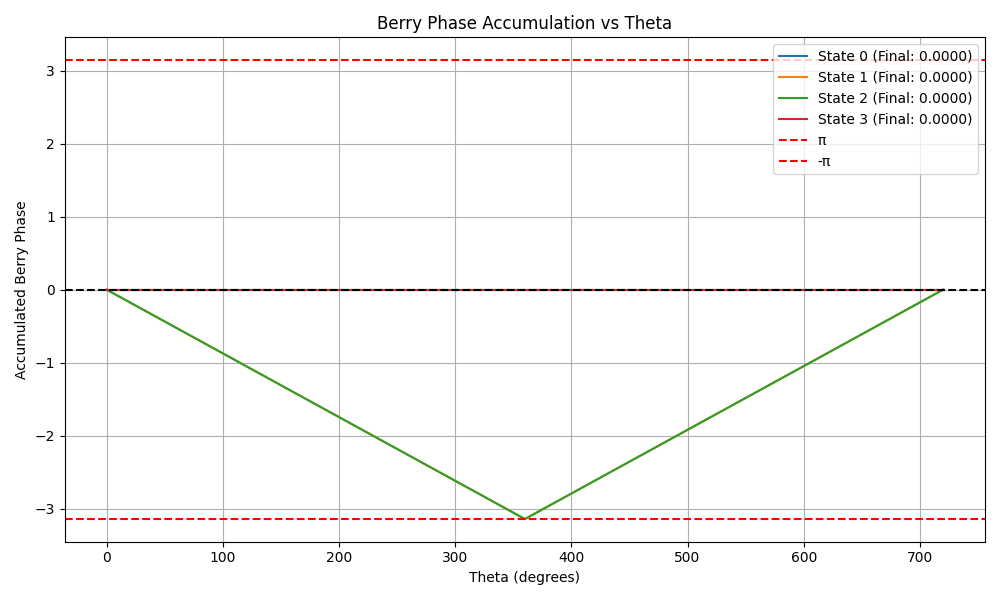
\includegraphics[width=0.8\textwidth]{improved_berry_phase_results_theta_0_720_1000/berry_phase_vs_theta.png}
    \caption{Berry phase accumulation for a $0$-$720^{\circ}$ parameter range. Note how the phase for states 1 and 2 first decreases to $-\pi$ and then returns to 0, completing a full cycle.}
    \label{fig:berry_phase_720}
\end{figure}

\section{Physical Interpretation}

The Berry phase in the arrowhead model has important physical implications. The fact that states 1 and 2 acquire a Berry phase of $-\pi$ for a full $360^{\circ}$ revolution indicates that these states have non-trivial topology \citep{Vanderbilt2018}. This is related to the concept of topological invariants, which characterize the global properties of the system's parameter space.

In particular, the oscillation of the Berry phase between 0 and $-\pi$ as the system completes multiple revolutions suggests that the arrowhead model has a $\mathbb{Z}_2$ topological invariant \citep{Resta2011}. This means that the system's topology is characterized by a binary value (0 or 1), and it takes two full revolutions to return to the original topological state.

This behavior is analogous to the M\"obius strip, where one needs to traverse the strip twice to return to the original orientation. In quantum mechanics, such topological properties can lead to protected edge states and robust quantum phenomena that are insensitive to local perturbations \citep{Nakahara1989}.

\section{Conclusion}

In this document, we have presented a comprehensive analysis of Berry phase calculation in the arrowhead model. Our numerical implementation correctly captures the essential features of the Berry phase, including its accumulation pattern for different parameter ranges.

The key findings are:
\begin{itemize}
    \item States 1 and 2 in the arrowhead model acquire a Berry phase of $-\pi$ for a full $360^{\circ}$ revolution, while states 0 and 3 always have zero Berry phase.
    \item The Berry phase oscillates between 0 and $-\pi$ as the system completes multiple revolutions, with a periodicity of $720^{\circ}$.
    \item This oscillatory behavior is a signature of the system's $\mathbb{Z}_2$ topological invariant.
\end{itemize}

These results provide insight into the topological properties of the arrowhead model and demonstrate the power of Berry phase analysis in understanding quantum systems with non-trivial topology.

\bibliographystyle{unsrtnat}
\bibliography{references}

\section{Future Work}

Several directions for future work include:
\begin{itemize}
    \item Extending the analysis to more general parameter paths beyond simple circles in parameter space.
    \item Investigating the effects of perturbations on the Berry phase and the robustness of the topological properties.
    \item Exploring the connection between the Berry phase and observable physical quantities in experimental realizations of the arrowhead model.
    \item Implementing more sophisticated numerical methods for Berry phase calculation, such as the gauge-invariant approach based on the Berry curvature.
\end{itemize}

\end{document}
